\PassOptionsToPackage{unicode=true}{hyperref} % options for packages loaded elsewhere
\PassOptionsToPackage{hyphens}{url}
%
\documentclass[ignorenonframetext,aspectratio=169]{beamer}
\usepackage{pgfpages}
\setbeamertemplate{caption}[numbered]
\setbeamertemplate{caption label separator}{: }
\setbeamercolor{caption name}{fg=normal text.fg}
\beamertemplatenavigationsymbolsempty
% Prevent slide breaks in the middle of a paragraph:
\widowpenalties 1 10000
\raggedbottom
\setbeamertemplate{part page}{
\centering
\begin{beamercolorbox}[sep=16pt,center]{part title}
  \usebeamerfont{part title}\insertpart\par
\end{beamercolorbox}
}
\setbeamertemplate{section page}{
\centering
\begin{beamercolorbox}[sep=12pt,center]{part title}
  \usebeamerfont{section title}\insertsection\par
\end{beamercolorbox}
}
\setbeamertemplate{subsection page}{
\centering
\begin{beamercolorbox}[sep=8pt,center]{part title}
  \usebeamerfont{subsection title}\insertsubsection\par
\end{beamercolorbox}
}
\AtBeginPart{
  \frame{\partpage}
}
\AtBeginSection{
  \ifbibliography
  \else
    \frame{\sectionpage}
  \fi
}
\AtBeginSubsection{
  \frame{\subsectionpage}
}
\usepackage{lmodern}
\usepackage{amssymb,amsmath}
\usepackage{ifxetex,ifluatex}
\usepackage{fixltx2e} % provides \textsubscript
\ifnum 0\ifxetex 1\fi\ifluatex 1\fi=0 % if pdftex
  \usepackage[T1]{fontenc}
  \usepackage[utf8]{inputenc}
  \usepackage{textcomp} % provides euro and other symbols
\else % if luatex or xelatex
  \usepackage{unicode-math}
  \defaultfontfeatures{Ligatures=TeX,Scale=MatchLowercase}
\fi
% use upquote if available, for straight quotes in verbatim environments
\IfFileExists{upquote.sty}{\usepackage{upquote}}{}
% use microtype if available
\IfFileExists{microtype.sty}{%
\usepackage[]{microtype}
\UseMicrotypeSet[protrusion]{basicmath} % disable protrusion for tt fonts
}{}
\IfFileExists{parskip.sty}{%
\usepackage{parskip}
}{% else
\setlength{\parindent}{0pt}
\setlength{\parskip}{6pt plus 2pt minus 1pt}
}
\usepackage{hyperref}
\hypersetup{
            pdftitle={CS5014 Machine Learning},
            pdfauthor={Lei Fang},
            pdfborder={0 0 0},
            breaklinks=true}
\urlstyle{same}  % don't use monospace font for urls
\newif\ifbibliography
\usepackage{color}
\usepackage{fancyvrb}
\newcommand{\VerbBar}{|}
\newcommand{\VERB}{\Verb[commandchars=\\\{\}]}
\DefineVerbatimEnvironment{Highlighting}{Verbatim}{commandchars=\\\{\}}
% Add ',fontsize=\small' for more characters per line
\usepackage{framed}
\definecolor{shadecolor}{RGB}{248,248,248}
\newenvironment{Shaded}{\begin{snugshade}}{\end{snugshade}}
\newcommand{\AlertTok}[1]{\textcolor[rgb]{0.94,0.16,0.16}{#1}}
\newcommand{\AnnotationTok}[1]{\textcolor[rgb]{0.56,0.35,0.01}{\textbf{\textit{#1}}}}
\newcommand{\AttributeTok}[1]{\textcolor[rgb]{0.77,0.63,0.00}{#1}}
\newcommand{\BaseNTok}[1]{\textcolor[rgb]{0.00,0.00,0.81}{#1}}
\newcommand{\BuiltInTok}[1]{#1}
\newcommand{\CharTok}[1]{\textcolor[rgb]{0.31,0.60,0.02}{#1}}
\newcommand{\CommentTok}[1]{\textcolor[rgb]{0.56,0.35,0.01}{\textit{#1}}}
\newcommand{\CommentVarTok}[1]{\textcolor[rgb]{0.56,0.35,0.01}{\textbf{\textit{#1}}}}
\newcommand{\ConstantTok}[1]{\textcolor[rgb]{0.00,0.00,0.00}{#1}}
\newcommand{\ControlFlowTok}[1]{\textcolor[rgb]{0.13,0.29,0.53}{\textbf{#1}}}
\newcommand{\DataTypeTok}[1]{\textcolor[rgb]{0.13,0.29,0.53}{#1}}
\newcommand{\DecValTok}[1]{\textcolor[rgb]{0.00,0.00,0.81}{#1}}
\newcommand{\DocumentationTok}[1]{\textcolor[rgb]{0.56,0.35,0.01}{\textbf{\textit{#1}}}}
\newcommand{\ErrorTok}[1]{\textcolor[rgb]{0.64,0.00,0.00}{\textbf{#1}}}
\newcommand{\ExtensionTok}[1]{#1}
\newcommand{\FloatTok}[1]{\textcolor[rgb]{0.00,0.00,0.81}{#1}}
\newcommand{\FunctionTok}[1]{\textcolor[rgb]{0.00,0.00,0.00}{#1}}
\newcommand{\ImportTok}[1]{#1}
\newcommand{\InformationTok}[1]{\textcolor[rgb]{0.56,0.35,0.01}{\textbf{\textit{#1}}}}
\newcommand{\KeywordTok}[1]{\textcolor[rgb]{0.13,0.29,0.53}{\textbf{#1}}}
\newcommand{\NormalTok}[1]{#1}
\newcommand{\OperatorTok}[1]{\textcolor[rgb]{0.81,0.36,0.00}{\textbf{#1}}}
\newcommand{\OtherTok}[1]{\textcolor[rgb]{0.56,0.35,0.01}{#1}}
\newcommand{\PreprocessorTok}[1]{\textcolor[rgb]{0.56,0.35,0.01}{\textit{#1}}}
\newcommand{\RegionMarkerTok}[1]{#1}
\newcommand{\SpecialCharTok}[1]{\textcolor[rgb]{0.00,0.00,0.00}{#1}}
\newcommand{\SpecialStringTok}[1]{\textcolor[rgb]{0.31,0.60,0.02}{#1}}
\newcommand{\StringTok}[1]{\textcolor[rgb]{0.31,0.60,0.02}{#1}}
\newcommand{\VariableTok}[1]{\textcolor[rgb]{0.00,0.00,0.00}{#1}}
\newcommand{\VerbatimStringTok}[1]{\textcolor[rgb]{0.31,0.60,0.02}{#1}}
\newcommand{\WarningTok}[1]{\textcolor[rgb]{0.56,0.35,0.01}{\textbf{\textit{#1}}}}
\setlength{\emergencystretch}{3em}  % prevent overfull lines
\providecommand{\tightlist}{%
  \setlength{\itemsep}{0pt}\setlength{\parskip}{0pt}}
\setcounter{secnumdepth}{0}

% set default figure placement to htbp
\makeatletter
\def\fps@figure{htbp}
\makeatother

%\usepackage[latin1]{inputenc}

\usepackage{graphicx}
\usepackage{rotating}
%\setbeamertemplate{caption}[numbered]
\usepackage{hyperref}
\usepackage{caption}
\usepackage[normalem]{ulem}
%\mode<presentation>
\usepackage{wasysym}
\usepackage{amsmath}
\usepackage{mathtools}
\usepackage[skins,theorems]{tcolorbox}
% \usepackage[,dvipsnames]{xcolor}
\tcbset{highlight math style={enhanced,
  colframe=red,colback=white,arc=0pt,boxrule=1pt}}

\newcommand{\normal}[2]{\ensuremath{\mathcal{N}\left (#1,#2 \right )}}
\newcommand{\Gaussian}[3]{\ensuremath{\frac{1}{\sqrt{2\pi}#3}
\text{exp}\left \{-\frac{1}{2#3^2} (#1-#2)^2 \right \}}}
\newcommand{\argmax}{\operatornamewithlimits{argmax}}
\newcommand{\expo}[1]{\ensuremath{\text{exp}\left \{ #1 \right \}}}
\newcommand{\studentt}[4]{\ensuremath{\mathcal{T}_{#4}(#1,#2,#3)}}
\newcommand{\vv}[1]{\boldsymbol{#1}}
\newcommand{\Prb}{\ensuremath{\mathbb{P}}}
\newcommand{\studenttk}[4]{\ensuremath{\mathcal{T}_{#4}(#1,#2,#3)}}
\newcommand{\argmin}{\operatornamewithlimits{argmin}}
\newcommand{\NIG}{\mathcal{NIG}}
\newcommand{\N}{\mathcal{N}}
\newcommand{\T}{\mathcal{T}}
\newcommand{\IG}{\mathcal{IG}}
\newcommand{\IW}{\mathcal{IW}}
\newcommand{\NNIW}{\mathcal{NNIW}}
\newcommand{\vct}{\text{vec}}
\newcommand{\NN}{\mathcal{NN}}
\newcommand{\tr}{\text{tr}}
\newcommand{\di}[2]{\ensuremath{ #1^{(#2)}}}
\newcommand{\dd}[1]{\ensuremath{ #1^{(i)}}}
\newcommand{\Di}[2]{\ensuremath{ \vv{#1}^{(#2)}}}

\newcommand{\E}[1]{\ensuremath{\mathbb{E}[#1]}}
\newcommand{\Var}[1]{\mathrm{Var}[#1]}
\newcommand{\Cov}[2]{\mathrm{Cov}[#1,#2]}
\newcommand{\Cor}[2]{\mathrm{Cor}[#1,#2]}

\usepackage[]{algorithm2e}
% \setbeamertemplate{navigation symbols}{}
\usepackage{tcolorbox}


%\titlegraphic{\includegraphics[width=0.3\paperwidth]{\string~/Dropbox/teaching/clemson-academic.png}}
\titlegraphic{\includegraphics[width=0.1\paperwidth]{./figs/crest.pdf}}
\setbeamertemplate{title page}[empty]

\setbeamerfont{subtitle}{size=\small}

\setbeamercovered{transparent}

\definecolor{clemsonpurple}{HTML}{522D80}
\definecolor{stablue}{HTML}{0052cc}
\definecolor{stared}{HTML}{ff4d4d}
\definecolor{clemsonorange}{HTML}{F66733}
\newcommand{\empha}[1]{\textbf{\textcolor{stablue}{#1}}}
\setbeamercolor{frametitle}{fg=stablue,bg=white}
\setbeamercolor{title}{fg=stablue,bg=white}
\setbeamercolor{local structure}{fg=stablue}
\setbeamercolor{section in toc}{fg=stablue,bg=white}
\setbeamercolor{subsection in toc}{fg=stared,bg=white}
\setbeamercolor{item projected}{fg=stablue,bg=white}
\setbeamertemplate{itemize item}{\color{stablue}$\bullet$}
\setbeamertemplate{itemize subitem}{\color{stablue}\scriptsize{$\bullet$}}
\let\Tiny=\tiny

%\makeatletter
%\setbeamertemplate{footline}{%
%\leavevmode
%\vbox{\begin{beamercolorbox}[dp=1.25ex,ht=2.75ex]{fg=black}%
%  \hspace*{1em}\insertsectionhead%
%  \ifx\insertsubsectionhead\@empty\relax\else$\quad\mid\quad$\insertsubsectionhead\fi :
%  \end{beamercolorbox}%
%  }%
%}
%\makeatother

\setbeamercolor{footercl}{fg=white,bg=stablue}
\setbeamerfont{stafont}{size = \large}
\setbeamerfont{footerfont}{size = \tiny}
% \makeatother
% \setbeamertemplate{footline}
% {
%   \leavevmode%
%   \hbox{%
%   \begin{beamercolorbox}[wd=.5\paperwidth,ht=5ex,dp=1ex, left]{footercl}%
%     \usebeamerfont*{stafont}\hspace*{1ex}\insertshortinstitute
%   \end{beamercolorbox}%
%   \begin{beamercolorbox}[wd=.25\paperwidth,ht=5ex,dp=1ex,center]{footercl}%
%     \usebeamerfont*{footerfont}\insertshorttitle\hspace*{1ex} \insertframenumber{}
%   \end{beamercolorbox}%
%   \begin{beamercolorbox}[wd=.25\paperwidth,ht=5ex,dp=1ex,right]{footercl}%
%    \includegraphics[height=5ex]{stalogo.png}
%   \end{beamercolorbox}}%
%   \vskip0pt%
% }
% \makeatletter
\makeatletter
\setbeamertemplate{footline}
{
  \leavevmode%
  \hbox{%
  \fontsize{13}{13}\fontfamily{ppl}\selectfont
  \begin{beamercolorbox}[wd=.5\paperwidth,ht=2.25ex,dp=1ex,left]{footercl}%
    \usebeamerfont{author in head/foot}\hspace*{1ex}\insertshortinstitute
   \end{beamercolorbox}%
   \begin{beamercolorbox}[wd=.25\paperwidth,ht=2.25ex,dp=1ex,right]{footercl}%
    % \hfill\hfill\hfill\hfill\hfill\hfill\hfill\hfill\hfill\hfill
    \parbox{.25\paperwidth}{\fontfamily{cmss}\selectfont{\hfill\hfill \usebeamerfont{footerfont}\insertshorttitle~\insertframenumber{}}}
  \end{beamercolorbox}%
  \begin{beamercolorbox}[wd=.25\paperwidth,ht=2.25ex,dp=1ex,left]{footercl}%
    \parbox{.25\paperwidth}{\hfill\includegraphics[height=1cm]{./figs/stalogo.png}}% original: 2ex
  \end{beamercolorbox}}%
  \vskip0pt%
}
\makeatother

\setbeamertemplate{navigation symbols}{}

% \AtBeginDocument{\author[L. Fang]{Lei Fang} \institute[www.st-andrews.ac.uk]{School of Computer Science, University of St Andrews}}

% \newcommand{\Ffootline}{%                   %%defines a new command called \Ffootline
% %\insertshortauthor,                         %%puts the abbreviated form of the author's name in the left corner
% \insertshorttitle,
% \insertshortinstitute, 
% \insertshortdate %%puts the abbreviated form of the author's institution in the middle
% \hfill
% \insertsection,
% \insertframenumber/\inserttotalframenumber} %%includes the current slide number over the total slide number in the right corner
% \setbeamertemplate{footline}{%              %%sets the options for the footline
% \usebeamerfont{structure}                   %%uses the same fonts adopted for the structure of the presentation 
% \Tiny\hspace*{4mm} \Ffootline \hspace{4mm}  %%sets the size of the font to Tiny and includes the content of the \Ffootline
% }                                           %%command leaving a margin of 4mm to the right and left of the content.



\AtBeginPart{}
\AtBeginSection{}
\AtBeginSubsection{}
\AtBeginSubsubsection{}
\setlength{\emergencystretch}{0em}
\setlength{\parskip}{0pt}
\AtBeginDocument{\author[L. Fang]{Lei Fang} \title[L9 Nonlinear models]{CS5014 Machine Learning}\institute[www.st-andrews.ac.uk]{School of Computer Science, University of St Andrews}}
\newenvironment{cols}[1][]{}{}

\newenvironment{col}[1]{\begin{minipage}{#1}\ignorespaces}{%
\end{minipage}
\ifhmode\unskip\fi
\aftergroup\useignorespacesandallpars}

\def\useignorespacesandallpars#1\ignorespaces\fi{%
#1\fi\ignorespacesandallpars}

\makeatletter
\def\ignorespacesandallpars{%
  \@ifnextchar\par
    {\expandafter\ignorespacesandallpars\@gobble}%
    {}%
}
\makeatother

\title{CS5014 Machine Learning}
\providecommand{\subtitle}[1]{}
\subtitle{Lecture 9 Fixed basis expansion models}
\author{Lei Fang}
\date{Spring 2021}

\begin{document}
\frame{\titlepage}

\hypertarget{introduction}{%
\section{Introduction}\label{introduction}}

\begin{frame}{Poll result last time}
\protect\hypertarget{poll-result-last-time}{}

\begin{center}\includegraphics[width=0.8\linewidth]{./figs/lec6poll} \end{center}

\end{frame}

\begin{frame}{Response}
\protect\hypertarget{response}{}

Speed: interrupt me during the lecture if you think I am too fast

\begin{itemize}
\tightlist
\item
  very hard for me to gauge the speed
\item
  w/o visual clue, I do not know where to spend more/less time
\end{itemize}

\bigskip

Difficulty: for those who think this course is too easy (there were at
least 2 said so in the first poll)

\begin{itemize}
\tightlist
\item
  minority but still not ideal to you
\item
  I will add extra exercises and one relevant ML research paper at the
  end of each lecture
\item
  you can also talk to us for further reading/exercises
\item
  how much you get out from the course is up to you
\end{itemize}

\end{frame}

\begin{frame}{Response to comments}
\protect\hypertarget{response-to-comments}{}

Comment 1: \texttt{"little bit on the Hessian matrix"}

\begin{itemize}
\tightlist
\item
  \textbf{Response}: we will do it today
\end{itemize}

Comment 2: \texttt{"need help with all the maths"}

\begin{itemize}
\tightlist
\item
  \textbf{Response}: Kasim and I are running extra lab sessions in even
  weeks; bring your questions. Can also schedule meetings with me.
\end{itemize}

\end{frame}

\begin{frame}{Response to comments}
\protect\hypertarget{response-to-comments-1}{}

Commen 3:
\texttt{"SGD on slide 19 is confusing ... is it the gradient for an individual feature or data point"}

\begin{center}\includegraphics[width=0.75\linewidth]{./figs/sgdresponse} \end{center}

\end{frame}

\begin{frame}{}
\protect\hypertarget{section}{}

\textbf{Response}: Good confusion/question! It worths some further
discussions. Remember the total likelihood is
\[\mathcal{L}(\vv{\theta}) =\sum_{i=1}^m  \underbrace{\dd{y} \log \sigma^{(i)}+(1-\dd{y})\log(1-\sigma^{(i)})}_{\dd{l}(\vv{\theta})}= \sum_{i=1}^m \dd{l}(\vv{\theta}), \;\;\; \text{therefore}\]
\[\nabla_{\vv{\theta}}\mathcal{L} = \sum_{i=1}^m\nabla_{\vv{\theta}}\dd{l}\;\;\; \text{due to linearity of derivative: } \nabla\sum f_i(x) = \sum \nabla f_i(x)\]

\begin{itemize}
\tightlist
\item
  total gradient (LHS) is a sum of invidual gradients (of each data
  point \((i)\))
\item
  SGD uses \(\nabla_{\vv{\theta}}\dd{l}\) instead of
  \(\nabla_{\vv{\theta}}\mathcal{L}\) at each iteration
\item
  also note the notation for future reference

  \begin{itemize}
  \tightlist
  \item
    \textbf{superscript} \((i)\) (with ``\textbf{()}'') index data
    points, \(y^{(i)}, \Di{x}{i}, \di{l}{i}\) \textit{etc.}
  \item
    \textbf{subscript} \(j\) index features (w/o brackets)
    \(\vv{\theta}^T\Di{x}{i} = \sum_{j=1}^n \di{x_{j}}{i}\theta_j\)
  \end{itemize}
\end{itemize}

\end{frame}

\begin{frame}{}
\protect\hypertarget{section-1}{}

On the other hand, optimise w.r.t features (i.e.~descent each
\(\theta_j\) in turn) is an algorithm called \empha{coordinate descent}

\begin{itemize}
\tightlist
\item
  not particularly useful for linear regression or logistic regression

  \begin{itemize}
  \tightlist
  \item
    slower descent than gradient descent, why ?
  \item
    in fact descent by axis aligned directional derivatives (with the
    relevant partial derivatives entries)
  \end{itemize}
\item
  useful when \(\theta_i, \theta_j\) are coupled though

  \begin{itemize}
  \tightlist
  \item
    descent is easier for \(\theta_2\) if conditional on \(\theta_1\)
  \item
    vice versa
  \item
    numerically stabler than direct optimisation
  \end{itemize}
\item
  EM (Expectation Maximization) is an example

  \begin{itemize}
  \tightlist
  \item
    mixture models or Hidden Markov Models (HMMs)
  \item
    we will study it later
  \end{itemize}
\end{itemize}

\end{frame}

\begin{frame}{Plan for today}
\protect\hypertarget{plan-for-today}{}

Learning algorithm:

\begin{itemize}
\tightlist
\item
  demystify Hessian
\item
  cases for and against Newton's method
\item
  practical issues of gradients
\end{itemize}

\bigskip

Model:

\begin{itemize}
\tightlist
\item
  probabilistic view unifies classification and regression
\item
  fixed basis models: extends linear models to nonlinear modelss

  \begin{itemize}
  \tightlist
  \item
    but still linear models: only needs to transform your data
  \item
    functional space view
  \end{itemize}
\end{itemize}

\end{frame}

\begin{frame}{Vignette: second derivative or curvature}
\protect\hypertarget{vignette-second-derivative-or-curvature}{}

\begin{columns}

\begin{column}{0.7\textwidth}
First, recap on univariate quadratics: $f({x}) = ax^2$
\begin{itemize}
\item multivariate version: $f(\vv{x})= \vv{x}^T\vv{Ax}$
\item gradient: $f'=2ax$ ($\nabla_{\vv{x}}f=2\vv{x}^T\vv{A}$ for multivariate $\vv{x}$)
\item second derivative (Hessian): $f''=2a$  ($\nabla^2_{\vv{x}}f=\vv{H}(f)=2\vv{A}$)
\item btw: effects of adding $bx$ and $c$ terms to $f$? (shifting $f$ to another location; $f''$ doesn't change)
\end{itemize}

So what $f''$ really is ?

\begin{itemize}
\item \empha{curvature}: curviness a curve deviates from straight line
\begin{itemize}
\item large curvature $\rightarrow$ bendy curve
\item small curvature $\rightarrow$ flatter curve 
\end{itemize}
\item \empha{Hessian}? the multivariant version of curvature
\end{itemize}
    
\end{column}

\begin{column}{0.3\textwidth}

\begin{center}\includegraphics[width=1\linewidth]{lecture9_files/figure-beamer/unnamed-chunk-3-1} \end{center}
\end{column}
\end{columns}

\end{frame}

\begin{frame}{Vignette: directional curvature and Hessian}
\protect\hypertarget{vignette-directional-curvature-and-hessian}{}

\begin{columns}

\begin{column}{0.65\textwidth}
Hessian: multivariant curvature. how ?
$$\vv{u}^T\vv{H}\vv{u} \text{ is directional curvature}$$
if $\vv{u}\in R^2$ is a unit vector $||\vv{u}||_2^2=\vv{u}^T\vv{u}=1$ (represents a direction in the input space)
\bigskip

Example: $f(\vv{x}) = x_1^2+x_2^2$ or $\vv{A}= \vv{I}$; Hessian: $$\footnotesize \vv{H}=2\vv{I}=\begin{pmatrix} {2}& 0 \\0 & {2}\end{pmatrix}$$
\begin{itemize}
\item if $\textcolor{red}{\vv{u}_1} =[1,0]^T:$ $\vv{u}_1^T\vv{H}\vv{u}_1=2$ \textcolor{red}{horizontal curvature}
\item if $\textcolor{teal}{\vv{u}_2} =[0,1]^T:$ $\vv{u}_2^T\vv{H}\vv{u}_2=2$ \textcolor{teal}{vertical curvature}
\item actually, curvature is 2 for all directions! (expected as it is a circle)
$\vv{u}^T\vv{H}\vv{u}=2\vv{u}^T\vv{u}=2$
\end{itemize}
\end{column}

\begin{column}{0.35\textwidth}

\begin{center}\includegraphics[height=0.45\textheight]{lecture9_files/figure-beamer/unnamed-chunk-4-1} \end{center}

\begin{center}\includegraphics[height=0.4\textheight]{lecture9_files/figure-beamer/unnamed-chunk-5-1} \end{center}
\end{column}
\end{columns}

\end{frame}

\begin{frame}{Vignette: directional curvature and Hessian}
\protect\hypertarget{vignette-directional-curvature-and-hessian-1}{}

\begin{columns}

\begin{column}{0.6\textwidth}
Example: $f(\vv{x}) = 4x_1^2+x_2^2$ or $\vv{A}= \begin{bmatrix}4, 0\\0, 1\end{bmatrix}.$ 
Hessian: $\vv{H}=2\begin{bmatrix}4, 0\\0, 1\end{bmatrix}=\begin{bmatrix} {8}& 0 \\0 & {2}\end{bmatrix}$
\begin{itemize}
\item if $\textcolor{red}{\vv{u}_1} =[1,0]^T:$ $\vv{u}_1^T\vv{H}\vv{u}_1=8$ \textcolor{red}{horizontal curvature} (curvy)
\item if $\textcolor{teal}{\vv{u}_2} =[0,1]^T:$ $\vv{u}_2^T\vv{H}\vv{u}_2=2$ \textcolor{teal}{vertical curvature} (less curvy)
\item the curvature changes with directions now
$$\vv{u}^T\vv{H}\vv{u}$$ is not a constant
\end{itemize}
\end{column}

\begin{column}{0.4\textwidth}

\begin{center}\includegraphics[height=0.42\textheight]{lecture9_files/figure-beamer/unnamed-chunk-6-1} \end{center}

\begin{center}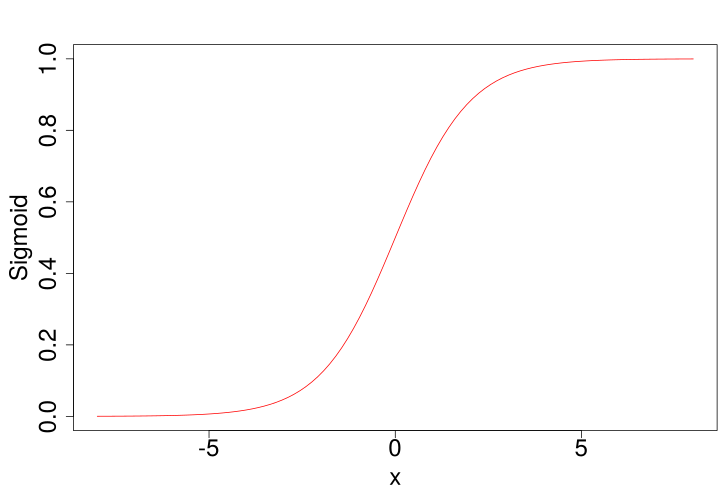
\includegraphics[height=0.42\textheight]{lecture9_files/figure-beamer/unnamed-chunk-7-1} \end{center}
\end{column}
\end{columns}

\end{frame}

\begin{frame}{Newton's direction and Hessian}
\protect\hypertarget{newtons-direction-and-hessian}{}

\begin{columns}

\begin{column}{0.75\textwidth}
Newton's method step: $$ \vv{\theta}_{t+1} \leftarrow \vv{\theta}_t -\underbrace{\vv{H}_t^{-1}\vv{g}_t}_{\vv{d}_t}$$

\begin{itemize}
\item Newton's direction: $\vv{d}_t = \vv{H}_t^{-1}\vv{g}_t$
\end{itemize}
 
  
Gradient descent step:  
  $$ \vv{\theta}_{t+1} \leftarrow \vv{\theta}_t -\alpha\vv{g}_t$$
  
Can you explain now
\begin{itemize}
 \item when $\vv{H}_t= \vv{I}$, $\vv{d}_t= \vv{g}_t$ ? what does it imply?
 \item the second case: $\vv{H}_t= \text{diag}(\{8,2\})$? 
\end{itemize}

Moral of the story? 
\begin{itemize}
 \item Shortcuts may not be ideal in long run. (very insightful !) 
\end{itemize}
\end{column}


\begin{column}{0.3\textwidth}

\begin{center}\includegraphics[height=0.35\textheight]{lecture9_files/figure-beamer/unnamed-chunk-8-1} \end{center}


\begin{center}\includegraphics[height=0.49\textheight]{lecture9_files/figure-beamer/unnamed-chunk-9-1} \end{center}
\end{column}
\end{columns}

\end{frame}

\begin{frame}{Newton's method for linear regression}
\protect\hypertarget{newtons-method-for-linear-regression}{}

Linear regression
\[\nabla_{\vv{\theta}}L= -2(\vv{y}-\vv{X\theta})^T\vv{X};\text{ and the Hessian is: } \nabla^2_{\vv{\theta}}L = 2\vv{X}^T\vv{X}\]

\begin{itemize}
\item
  constant Hessian matrix: the quadratic approximation is exact
\item
  Newton step: assume starting from any \(\vv{\theta}_0 \in R^n\)
  \begin{align*}\vv{\theta}_1 &\leftarrow \vv{\theta}_0 - \underbrace{(2\vv{X}^T\vv{X})^{-1}}_{\vv{H}^{-1}}\underbrace{ (-2\vv{X}^T(\vv{y}-\vv{X\theta}_0) )}_{\vv{g}_0} \\
   \vv{\theta}_1 &\leftarrow \vv{\theta}_0 + (\vv{X}^T\vv{X})^{-1}(\vv{X}^T\vv{y} -\vv{X}^T\vv{X}\vv{\theta}_0) =  \underbrace{(\vv{X}^T\vv{X})^{-1}\vv{X}^T\vv{y}}_{\vv{\theta}_{ls}: \text{ one step optimised}}
    \end{align*}
\item
  why \(\vv{\theta}_{ls}\) is a minimum ? \(\vv{H}= 2\vv{X}^T\vv{X}\) is
  positive definite (similar to univariate function).
\end{itemize}

\footnotesize  for all \(\vv{u}\neq \vv{0}\),
\(\vv{u}^T\vv{H}\vv{u}=2\underbrace{\vv{u}^T\vv{X}^T}_{\vv{v}^T}\underbrace{\vv{X}\vv{u}}_{\vv{v}}= 2\vv{v}^T\vv{v}>0\)
(vector's norm is always positive).

\footnotesize useful identities to find the Hessian:
\(\frac{\partial \vv{x}^T \vv{A}}{\partial \vv{x}} = \vv{A}^{T}, \frac{\partial \vv{Ax}}{\partial \vv{x}} = \vv{A}\)

\end{frame}

\begin{frame}{Newton's method for logistic regression (code on studres)}
\protect\hypertarget{newtons-method-for-logistic-regression-code-on-studres}{}

\begin{center}\includegraphics[width=1\linewidth]{lecture9_files/figure-beamer/unnamed-chunk-11-1} \end{center}

\end{frame}

\begin{frame}{A closer look: Newton's method for logistic regression}
\protect\hypertarget{a-closer-look-newtons-method-for-logistic-regression}{}

\begin{cols}

\begin{col}{0.55\textwidth}

Gradient descent: zig-zagging

\begin{itemize}
\tightlist
\item
  consecutive gradients are perpendicular

  \begin{itemize}
  \tightlist
  \item
    doesn't look so because of plotting ratio
  \end{itemize}
\item
  zig-zagging in a narrow valley
\end{itemize}

Newton's method

\begin{itemize}
\tightlist
\item
  converge faster
\item
  does starting point matter?
\item
  what if we start from top right corner ?

  \begin{itemize}
  \tightlist
  \item
    can you envision the cost function from the contour ?
  \end{itemize}
\end{itemize}

\begin{tcolorbox}[colback=green!5,colframe=green!40!black]
\footnotesize
All code to generate the figs/algorithms on studres
\begin{itemize}
\item in R at the moment; 
\item will translate to Python
\end{itemize}
\end{tcolorbox}

\end{col}

\begin{col}{0.45\textwidth}

\begin{center}\includegraphics[width=1\linewidth]{lecture9_files/figure-beamer/unnamed-chunk-12-1} \end{center}

\end{col}

\end{cols}

\end{frame}

\begin{frame}{Why not everyone is Newton in ML then?}
\protect\hypertarget{why-not-everyone-is-newton-in-ml-then}{}

\begin{cols}

\begin{col}{0.70\textwidth}

Newton's method can diverge

\begin{itemize}
\tightlist
\item
  bad quadratic approximation (top fig)
\item
  might approximate a downward facing bowl (btm fig)

  \begin{itemize}
  \tightlist
  \item
    finding maximum instead !
  \item
    Newton's direction can either descent or ascent

    \begin{itemize}
    \tightlist
    \item
      depends on the local approximation
    \item
      need to check the Hessian for the lost function
    \end{itemize}
  \end{itemize}
\end{itemize}

Remedy

\begin{itemize}
\tightlist
\item
  apply some learning rate \(\alpha'<1\) rather than exact Newton step:
  \(\vv{\theta} \leftarrow \vv{\theta}_t -\alpha'\vv{H}_t^{-1}\vv{g}_t\)

  \begin{itemize}
  \tightlist
  \item
    line search to find \(\alpha'\): even simply grid search in
    \((0,1]\):
    \[\alpha' \leftarrow \argmin_{\alpha} L(\vv{\theta}_t -\alpha \vv{d}_t)\]
  \end{itemize}
\item
  or use gradient descent first; then Newton's method to speed up at the
  end
\end{itemize}

\end{col}

\begin{col}{0.30\textwidth}

\begin{center}\includegraphics[width=1\linewidth]{lecture9_files/figure-beamer/unnamed-chunk-13-1} \end{center}

\begin{center}\includegraphics[width=1\linewidth]{./figs/newtonsMethodNonConvex} \end{center}

\end{col}

\end{cols}

\end{frame}

\begin{frame}{Why not everyone is Newton in ML then?}
\protect\hypertarget{why-not-everyone-is-newton-in-ml-then-1}{}

Newton's method is expensive

\begin{itemize}
\tightlist
\item
  Hessian: \(n\times n\) derivatives to compute
\item
  matrix is very expensive to invert in general
\end{itemize}

\bigskip

Hessian can be impossible to invert

\begin{itemize}
\tightlist
\item
  singular matrix (\(\vv{H}^{-1}\) does not exist), similar to divide a
  number by \(0\)
\item
  \emph{regularisation} is useful (adding small constants to diagonal
  entries)

  \begin{itemize}
  \tightlist
  \item
    I have used 0.01 in my Newton's algorithm above
  \end{itemize}
\item
  stochastic Newton's method ?

  \begin{itemize}
  \tightlist
  \item
    inverting a rank one matrix ! (\(\dd{\vv{x}}(\dd{\vv{x}})^T\) is
    rank 1, so singular)
  \item
    in human language: cannot estimate the curvature realiably with only
    one data
  \end{itemize}
\end{itemize}

\end{frame}

\hypertarget{r-librarydplyr-warn.conflicts-false-norm---functionx-x-sqrtsumx2-sinv---solves-i-know-i-said-not-to-do-this-step1---functionmu-alpha-1-d---sweepx-2-mu---score---colsumsd-norm-mu-alpha-dropsinv-score-steep---functionmu-n-10-...-results---vectorlist-length-n-fori-in-seq_lenn-resultsi---step1mu-...-mu---resultsi-results-m---do.callrbind-steepc-5--2-8-m---rbindc-5--2-m-parmar-c4.5-4.5-1-1-contourxg-yg-z-nlevels-40-xlab-expressionmu1-ylab-expressionmu2-ablineh-0-v-0-lty-2-pointsm-pch-20-type-b---}{%
\section{\texorpdfstring{\texttt{\{r\}\ \#\ library(dplyr,\ warn.conflicts\ =\ FALSE)\ \#\ norm\ \textless{}-\ function(x)\ x\ /\ sqrt(sum(x\^{}2))\ \#\ Sinv\ \textless{}-\ solve(S)\ \ \#\#\ I\ know\ I\ said\ not\ to\ do\ this!\ \#\ step1\ \textless{}-\ function(mu,\ alpha\ =\ 1)\ \{\ \#\ \ \ \ \ \ \ \ \ D\ \textless{}-\ sweep(x,\ 2,\ mu,\ "-")\ \#\ \ \ \ \ \ \ \ \ score\ \textless{}-\ colSums(D)\ \%\textgreater{}\%\ norm\ \#\ \ \ \ \ \ \ \ \ mu\ +\ alpha\ *\ drop(Sinv\ \%*\%\ score)\ \#\ \}\ \#\ steep\ \textless{}-\ function(mu,\ n\ =\ 10,\ ...)\ \{\ \#\ \ \ \ \ \ \ \ \ results\ \textless{}-\ vector("list",\ length\ =\ n)\ \#\ \ \ \ \ \ \ \ \ for(i\ in\ seq\_len(n))\ \{\ \#\ \ \ \ \ \ \ \ \ \ \ \ \ \ \ \ \ results{[}{[}i{]}{]}\ \textless{}-\ step1(mu,\ ...)\ \#\ \ \ \ \ \ \ \ \ \ \ \ \ \ \ \ \ mu\ \textless{}-\ results{[}{[}i{]}{]}\ \#\ \ \ \ \ \ \ \ \ \}\ \#\ \ \ \ \ \ \ \ \ results\ \#\ \}\ \#\ m\ \textless{}-\ do.call("rbind",\ steep(c(-5,\ -2),\ 8))\ \#\ m\ \textless{}-\ rbind(c(-5,\ -2),\ m)\ \#\ \ \#\ par(mar\ =\ c(4.5,\ 4.5,\ 1,\ 1))\ \#\ contour(xg,\ yg,\ z,\ nlevels\ =\ 40,\ xlab\ =\ expression(mu{[}1{]}),\ \ \#\ \ \ \ \ \ \ \ \ ylab\ =\ expression(mu{[}2{]}))\ \#\ abline(h\ =\ 0,\ v\ =\ 0,\ lty\ =\ 2)\ \#\ points(m,\ pch\ =\ 20,\ type\ =\ "b")\ \textless{}!-\/-}
--\textgreater{}}{\{r\} \# library(dplyr, warn.conflicts = FALSE) \# norm \textless{}- function(x) x / sqrt(sum(x\^{}2)) \# Sinv \textless{}- solve(S)  \#\# I know I said not to do this! \# step1 \textless{}- function(mu, alpha = 1) \{ \#         D \textless{}- sweep(x, 2, mu, "-") \#         score \textless{}- colSums(D) \%\textgreater{}\% norm \#         mu + alpha * drop(Sinv \%*\% score) \# \} \# steep \textless{}- function(mu, n = 10, ...) \{ \#         results \textless{}- vector("list", length = n) \#         for(i in seq\_len(n)) \{ \#                 results{[}{[}i{]}{]} \textless{}- step1(mu, ...) \#                 mu \textless{}- results{[}{[}i{]}{]} \#         \} \#         results \# \} \# m \textless{}- do.call("rbind", steep(c(-5, -2), 8)) \# m \textless{}- rbind(c(-5, -2), m) \#  \# par(mar = c(4.5, 4.5, 1, 1)) \# contour(xg, yg, z, nlevels = 40, xlab = expression(mu{[}1{]}),  \#         ylab = expression(mu{[}2{]})) \# abline(h = 0, v = 0, lty = 2) \# points(m, pch = 20, type = "b") \textless{}!-\/- --\textgreater{}}}\label{r-librarydplyr-warn.conflicts-false-norm---functionx-x-sqrtsumx2-sinv---solves-i-know-i-said-not-to-do-this-step1---functionmu-alpha-1-d---sweepx-2-mu---score---colsumsd-norm-mu-alpha-dropsinv-score-steep---functionmu-n-10-...-results---vectorlist-length-n-fori-in-seq_lenn-resultsi---step1mu-...-mu---resultsi-results-m---do.callrbind-steepc-5--2-8-m---rbindc-5--2-m-parmar-c4.5-4.5-1-1-contourxg-yg-z-nlevels-40-xlab-expressionmu1-ylab-expressionmu2-ablineh-0-v-0-lty-2-pointsm-pch-20-type-b---}}

\begin{frame}{Quasi-Newton (Newton-like methods)}
\protect\hypertarget{quasi-newton-newton-like-methods}{}

Quasi-Newton: approximate \(\vv{H}_t\) (or even \(\vv{H}_t^{-1}\)
directly) instead

\begin{itemize}
\tightlist
\item
  some crude Hessian approximations work

  \begin{itemize}
  \tightlist
  \item
    gradient descent is one! \(\vv{H}_t=?\)
  \item
    some people use diagonal approximation matrix for \(\vv{H}_t\)

    \begin{itemize}
    \tightlist
    \item
      might perform well actually, what does it imply though ?
    \end{itemize}
  \end{itemize}
\item
  Broyden-Fletcher-Goldfarb-Shanno algorithm (BFGS) is more advanced

  \begin{itemize}
  \tightlist
  \item
    approximate Hessian by previous gradients
  \item
    very widely used optimisation routine (Python, R, Matlab, Julia all
    have its implementation)
  \item
    L-BFGS is limited memory version (do not use all the gradient
    history)
  \end{itemize}
\end{itemize}

\end{frame}

\begin{frame}{Gradients in real life}
\protect\hypertarget{gradients-in-real-life}{}

\begin{tcolorbox}[colback=green!5,colframe=green!40!black, title=A Burning Question]
\centering how to find out the gradient and Hessian for a new loss $L(\vv{\theta})$?
\end{tcolorbox}

Option 1: manual derivation: a lot of ML researchers do it this way

\footnotesize

\begin{itemize}
\tightlist
\item
  method 1: use vector differentiation identities if you can (more
  efficient for implementation: vectorisation)
\end{itemize}

\footnotesize   \[\frac{1}{2m}L(\vv{\theta})=\frac{1}{2m}(\vv{y}-\vv{X\theta})^T(\vv{y}-\vv{X\theta}) \Rightarrow  \frac{1}{2m}\nabla_{\vv{\theta}}L=\frac{1}{2m} \underbrace{\nabla_{\vv{y}-\vv{X\theta}}(\vv{y}-\vv{X\theta})^T(\vv{y}-\vv{X\theta})}_{2(\vv{y}-\vv{X\theta})^T}\cdot \underbrace{\nabla_{\vv{\theta}} (\vv{y}-\vv{X\theta})}_{-\vv{X}}\]

\begin{itemize}
\tightlist
\item
  method 2: or break down the total loss as a sum of individual losses;
  then sum up
\end{itemize}

\footnotesize  \[\frac{1}{2m}L(\vv{\theta})=\frac{1}{2m}\sum_{i=1}^m \underbrace{(\dd{y}-\vv{\theta}^T\Di{x}{i})^2}_{\dd{l}(\vv{\theta})} \Rightarrow  \nabla_{\vv{\theta}}\dd{l}=2(\dd{y}-\vv{\theta}^T\Di{x}{i})(-\Di{x}{i})^T\]

\end{frame}

\begin{frame}{Vector calculus shapes}
\protect\hypertarget{vector-calculus-shapes}{}

\begin{cols}

\begin{col}{0.62\textwidth}

\renewcommand{\arraystretch}{2}
\begin{tabular}{cccc}
& & Scalar & Vector \\
& & $x$ & $\vv{x}$ \\
\hline
Scalar & $y$ & {\Large $\frac{\partial y}{\partial x}$} (scalar) &{\Large $\frac{\partial y}{\partial \vv{x}}$} (row vector)\\
Vector & $\vv{y}$ &{\Large $\frac{\partial \vv{y}}{\partial x}$} (column vector) &{\Large $\frac{\partial \vv{y}}{\partial \vv{x}}$} (matrix)\\
\hline
\end{tabular}
\bigskip

\begin{itemize}
\tightlist
\item
  notation: vectors are bold font letters, e.g. \(\vv{x}\)
\item
  we use numerator notation here (easier to apply chain rule)

  \begin{itemize}
  \tightlist
  \item
    scalar \(y\)'s gradient is a row vector, i.e.
    \(\frac{\partial y}{\partial \vv{x}}\)
  \item
    vector \(\vv{y}\)'s derivative is a column vector, i.e.
    \(\frac{\partial \vv{y}}{\partial x}\)
  \end{itemize}
\end{itemize}

\end{col}

\begin{col}{0.38\textwidth}

\[\frac{\partial y}{\partial \vv{x}} = \begin{bmatrix}\frac{\partial y}{\partial {x}_1}& \frac{\partial y}{\partial {x}_2} &\ldots&\frac{\partial y}{\partial {x}_n}\end{bmatrix}\]

\[\footnotesize \frac{\partial \vv{y}}{\partial {x}} = \begin{bmatrix}\frac{\partial y_1}{\partial {x}} \\ \frac{\partial y_2}{\partial {x}} \\\vdots \\ \frac{\partial y_m}{\partial {x}}\end{bmatrix}\]
\[\footnotesize \frac{\partial \vv{y}}{\partial \vv{x}} = \begin{bmatrix}\frac{\partial y_1}{\partial \vv{x}}\\ \frac{\partial y_2}{\partial \vv{x}}\\ \vdots \\ \frac{\partial y_m}{\partial \vv{x}} \end{bmatrix}=  \begin{bmatrix}\frac{\partial y_1}{\partial {x}_1}& \frac{\partial y_1}{\partial {x}_2}& \ldots&\frac{\partial y_1}{\partial {x}_n}\\ \frac{\partial y_2}{\partial {x}_1}& \frac{\partial y_2}{\partial {x}_2}& \ldots&\frac{\partial y_2}{\partial {x}_n}\\ \vdots & \vdots& \ddots &\vdots \\ \frac{\partial y_m}{\partial {x}_1}& \frac{\partial y_m}{\partial {x}_2}& \ldots&\frac{\partial y_m}{\partial {x}_n} \end{bmatrix}\]

\end{col}

\end{cols}

\end{frame}

\begin{frame}{Check your gradients before use}
\protect\hypertarget{check-your-gradients-before-use}{}

Good coding practice apply in ML as well: testing testing testing
\[\vv{u}^T\nabla_{\vv{\theta}}L(\vv{\theta}) \approx \frac{1}{2\epsilon} (L(\vv{\theta}+\epsilon \vv{u})-L(\vv{\theta}-\epsilon \vv{u}))\]

\begin{itemize}
\tightlist
\item
  check your derivation against the above rule\\
\item
  for some small \(\epsilon = 10^{-5}\) etc.
\item
  \(\vv{u}\) can be standard basis directions i.e.
  \([1,0,0,\ldots]^T, [0,1,0,\ldots]^T\)
\end{itemize}

\end{frame}

\begin{frame}{Gradients in real life}
\protect\hypertarget{gradients-in-real-life-1}{}

\[\frac{\partial L(\theta_j)}{\partial \theta_j} \approx \frac{1}{2\epsilon} (L({\theta_j}+\epsilon )-L({\theta_j}-\epsilon ))\]

Option 2: finite difference approximation

\begin{itemize}
\tightlist
\item
  use approximated finite difference instead
\item
  to evaluate gradient at \(\vv{\theta}_t\),

  \begin{itemize}
  \tightlist
  \item
    choose small \(\epsilon = 10^{-5}\)
  \item
    perturb each dimension in turn to find partial derivatives
  \end{itemize}
\item
  not practical for large model (esp.~evaluation of \(L\) is expensive)
\item
  subject to truncation error
\item
  default choice for \texttt{scipy.optimize} method: approximation done
  for you
\end{itemize}

\end{frame}

\begin{frame}{Gradients in real life}
\protect\hypertarget{gradients-in-real-life-2}{}

Option 3: auto differentiation

\begin{itemize}
\tightlist
\item
  an active (and old) research area in computing and ML

  \begin{itemize}
  \tightlist
  \item
    nobody enjoy doing derivatives by hand \ldots{}
  \end{itemize}
\item
  input: a function; output: gradient function
\item
  use computation graph (like Neural Nets) to speed up/keep track the
  calculation
\item
  backpropagation is one example
\item
  a lot of packages out there: autograd in Python, PyTorch etc.
\end{itemize}

\end{frame}

\begin{frame}[fragile]{Example of autograd for logistic regression}
\protect\hypertarget{example-of-autograd-for-logistic-regression}{}

\tiny

\begin{Shaded}
\begin{Highlighting}[]
\ImportTok{import}\NormalTok{ autograd.numpy }\ImportTok{as}\NormalTok{ np}
\ImportTok{from}\NormalTok{ autograd }\ImportTok{import}\NormalTok{ grad}

\KeywordTok{def}\NormalTok{ logistic_predictions(weights, inputs):}
    \CommentTok{# Outputs probability of a label being true according to logistic model.}
    \ControlFlowTok{return}\NormalTok{ sigmoid(np.dot(inputs, weights))}

\KeywordTok{def}\NormalTok{ training_loss(weights):}
    \CommentTok{# Training loss is the negative log-likelihood of the training labels.}
\NormalTok{    preds }\OperatorTok{=}\NormalTok{ logistic_predictions(weights, inputs)}
\NormalTok{    label_probabilities }\OperatorTok{=}\NormalTok{ np.log(preds) }\OperatorTok{*}\NormalTok{ targets }\OperatorTok{+}\NormalTok{ np.log((}\DecValTok{1} \OperatorTok{-}\NormalTok{ preds)) }\OperatorTok{*}\NormalTok{ (}\DecValTok{1} \OperatorTok{-}\NormalTok{ targets)}
    \ControlFlowTok{return} \OperatorTok{-}\NormalTok{np.}\BuiltInTok{sum}\NormalTok{(label_probabilities)}

\CommentTok{# Define a function that returns gradients of training loss using Autograd.}
\NormalTok{training_gradient_fun }\OperatorTok{=}\NormalTok{ grad(training_loss)}

\CommentTok{# Optimize weights using gradient descent.}
\NormalTok{weights }\OperatorTok{=}\NormalTok{ np.array([}\FloatTok{0.0}\NormalTok{, }\FloatTok{0.0}\NormalTok{, }\FloatTok{0.0}\NormalTok{])}
\BuiltInTok{print}\NormalTok{(}\StringTok{"Initial loss:"}\NormalTok{, training_loss(weights))}
\ControlFlowTok{for}\NormalTok{ i }\KeywordTok{in} \BuiltInTok{range}\NormalTok{(}\DecValTok{100}\NormalTok{):}
\NormalTok{    weights }\OperatorTok{-=}\NormalTok{ training_gradient_fun(weights) }\OperatorTok{*} \FloatTok{0.01}

\BuiltInTok{print}\NormalTok{(}\StringTok{"Trained loss:"}\NormalTok{, training_loss(weights))}
\end{Highlighting}
\end{Shaded}

\end{frame}

\begin{frame}{Towards nonlinear models: regression}
\protect\hypertarget{towards-nonlinear-models-regression}{}

\begin{cols}

\begin{col}{0.70\textwidth}

For linear regression:

\[ P({y}|{\vv{x}}, \vv{\theta}) = N(\underbrace{f({\vv{x}};\vv{\theta})}_{\vv{\theta}^T{\vv{x}}: \text{ linear}}, \sigma^2) \;\text{or }\; y= \underbrace{f(\vv{x};\vv{\theta})}_{\vv{\theta}^T{\vv{x}}} +\vv{\epsilon}, \;\; \dd{\epsilon}\sim N(0, \sigma^2)\]

The regression function \(f\) is assumed linear
\[f(\vv{x};\vv{\theta}) = \vv{\theta}^T{\vv{x}}\]

\begin{itemize}
\tightlist
\item
  \emph{i.e.} fitting lines/hyperplanes
\item
  in real life, a lot of relationships are not linear
\item
  and we do not know what \(f(\vv{x})\) should look like !
\end{itemize}

\end{col}

\begin{col}{0.30\textwidth}

\begin{center}\includegraphics[height=0.42\textheight]{lecture9_files/figure-beamer/unnamed-chunk-16-1} \end{center}

\begin{center}\includegraphics[height=0.45\textheight]{lecture9_files/figure-beamer/unnamed-chunk-17-1} \end{center}

\end{col}

\end{cols}

\end{frame}

\begin{frame}{Towards nonlinear models: classification}
\protect\hypertarget{towards-nonlinear-models-classification}{}

\begin{cols}

\begin{col}{0.70\textwidth}

For logistic regression:

\[P({y}|{\vv{x}}, \vv{\theta}) = \text{Ber}(\sigma(\underbrace{f(\vv{x};\vv{\theta})}_{\vv{\theta}^T{\vv{x}}: \text{ linear}})= \sigma^{{y}}(1-\sigma)^{(1-{{y}})}\]
To predict the label \(y\) for any input \(\vv{x}\):
\begin{align*}\footnotesize
{y}=1\; \text{if }P({{y}}=1|{\vv{x}}, \vv{\theta}) > 0.5\;\;  {y}=0\; \text{if otherwise}
\end{align*}

Note that the \textbf{decision boundary} is linear (hyperplane or line)

\[P({{y}}=1|{\vv{x}}, \vv{\theta}) = 0.5 \Rightarrow \vv{\theta}^T\vv{x} =0\]

\begin{itemize}
\tightlist
\item
  \(i.e.\) separating data by lines/hyperplanes
\item
  in reality, we do know what \(f\) should be; plane or a more general
  surface
\end{itemize}

\end{col}

\begin{col}{0.30\textwidth}

\begin{center}\includegraphics[width=0.95\linewidth]{lecture9_files/figure-beamer/unnamed-chunk-18-1} \end{center}

\begin{center}\includegraphics[width=0.95\linewidth]{lecture9_files/figure-beamer/unnamed-chunk-19-1} \end{center}

\end{col}

\end{cols}

\end{frame}

\begin{frame}{Nonlinear classification data}
\protect\hypertarget{nonlinear-classification-data}{}

\begin{cols}

\begin{col}{0.70\textwidth}

What if your data looks like this ?

\begin{itemize}
\tightlist
\item
  no linear descision boudary or
  \(f(\vv{x};\vv{\theta}) = \vv{\theta}^T\vv{x}\) seems making much
  sense
\item
  but a non-linear boundary makes more sense

  \begin{itemize}
  \tightlist
  \item
    the classification rule is actually
    \(||\vv{x}||_2^2 = x_1^2+x_2^2\leq 1\)
  \item
    distance to \(\vv{0}\) is less than 1
  \item
    the boundary is a circle
  \item
    \footnotesize I know it because I generated the data
  \end{itemize}
\end{itemize}

\end{col}

\begin{col}{0.30\textwidth}

\begin{center}\includegraphics[height=0.45\textheight]{lecture9_files/figure-beamer/unnamed-chunk-20-1} \end{center}

\begin{center}\includegraphics[height=0.45\textheight]{lecture9_files/figure-beamer/unnamed-chunk-21-1} \end{center}

\end{col}

\end{cols}

\end{frame}

\begin{frame}{Nonlinear model: polynomial model}
\protect\hypertarget{nonlinear-model-polynomial-model}{}

\begin{center}\includegraphics[height=0.4\textheight]{lecture9_files/figure-beamer/figures-side-1} \includegraphics[height=0.4\textheight]{lecture9_files/figure-beamer/figures-side-2} \end{center}

Both models are actually 2nd order polynomial:
\footnotesize\[f(\vv{x};\vv{\beta}) = \beta_0+ \beta_1x_1+ \beta_2x_2 +\beta_3x_1x_2+\beta_4x_1^2 +\beta_5x_2^2 =\sum_{k=0}^5 \beta_j \phi_j(\vv{x})=\vv{\beta}^T\vv{\phi}(\vv{x})\]

\normalsize

\begin{itemize}
\item
  where
  \[\footnotesize \vv{\phi}(\vv{x}) = [\underbrace{1}_{\phi_0(\vv{x})}, \underbrace{x_1}_{\phi_1(\vv{x})}, \underbrace{x_2}_{\phi_2(\vv{x})}, \underbrace{x_1x_2}_{\phi_3(\vv{x})}, \underbrace{x_1^2}_{\phi_4(\vv{x})}, \underbrace{x_2^2}_{\phi_5(\vv{x})}]^T\]
\item
  it expands \(\vv{x}=[1, x_1, x_2]^T\) to a larger vector
\end{itemize}

\end{frame}

\begin{frame}{Nonlinear response from linear model}
\protect\hypertarget{nonlinear-response-from-linear-model}{}

Note that you get a free nonlinear model by transforming the input
\(\vv{X}\)
\[\footnotesize \vv{X} = \begin{bmatrix} 1& \di{x}{1}_1& \di{x}{1}_2 \\
1& \di{x}{2}_1& \di{x}{2}_2 \\
\vdots& \vdots& \vdots \\
1 &  \di{x}{m}_1& \di{x}{m}_2
\end{bmatrix} \Rightarrow \vv{\Phi} =\begin{bmatrix} \vv{\phi}(\Di{x}{1}) \\
\vv{\phi}(\Di{x}{2}) \\
\vdots \\
\vv{\phi}(\Di{x}{m})
\end{bmatrix} = \begin{bmatrix} 1& \di{x}{1}_1& \di{x}{1}_2& \di{x}{1}_1 \di{x}{1}_2& (\di{x}{1}_1)^2 & (\di{x}{1}_2)^2\\
1& \di{x}{2}_1& \di{x}{2}_2& \di{x}{2}_1 \di{x}{2}_2& (\di{x}{2}_1)^2 & (\di{x}{2}_2)^2\\
\vdots& \vdots& \vdots & \vdots & \vdots & \vdots\\
1& \di{x}{m}_1& \di{x}{m}_2& \di{x}{m}_1 \di{x}{m}_2& (\di{x}{m}_1)^2 & (\di{x}{m}_2)^2\\
\end{bmatrix}\]

\begin{itemize}
\tightlist
\item
  remember superscript \((i)\) index data samples; and subscript index
  features
\item
  \(\vv{\Phi}\) is a \(m\times 6\) matrix
\item
  for higher order polynormial, the new design matrix just gets wider
\end{itemize}

\normalsize

The expanded model for regression is
\[\vv{y} = \vv{\Phi}\vv{\beta} + \vv{\epsilon}\]

\begin{itemize}
\tightlist
\item
  still a linear model w.r.t \(\vv{\phi}\), the expanded new features
\item
  all existing results apply: gradient descent, normal equation (replace
  \(\vv{X}\) with \(\vv{\Phi}\))
  \[\vv{\beta}_{ls} =(\vv{\Phi}^T\vv{\Phi})^{-1}\vv{\Phi}^T\vv{y}\]
\end{itemize}

\end{frame}

\begin{frame}{General basis function expansion}
\protect\hypertarget{general-basis-function-expansion}{}

It turns out \(\vv{\phi}{(\vv{x})}\) can take a wide range of forms

\begin{itemize}
\tightlist
\item
  each \(\phi_k(\vv{x})\) is a \(R^n\rightarrow R\) transformation; so
  \(\vv{\phi}\) is a \(R^n\rightarrow R^p\) transformation

  \begin{itemize}
  \tightlist
  \item
    previous example: \(n=3\), \(p=6\)
  \end{itemize}
\item
  obviously, if \(\vv{\phi}(\vv{x}) = \vv{I}\vv{x}\), we recover
  ordinary linear regression
\item
  previous case: \(\phi_k(\vv{x}) = x_j^2\), \(x_jx_{j'}\), \(x_j\), or
  1, for 2-nd order polynormial
\item
  3-rd order polynomial will add \(\phi_k(\vv{x}) = x_j^3\),
  \(x_jx_{j'}x_{j''}\) on top
\item
  \(\phi_k(\vv{x}) = \log(x_j), \sqrt{x_j}, \sigma(x_j+\mu)\; (\text{sigmoid function}), \ldots\)
\item
  radial basis function:
  \(\phi_k(\vv{x}) = \exp\left (-\frac{||\vv{x}-\vv{\mu}_k||_2^2}{2s^2}\right )\)
\end{itemize}

\begin{center}\includegraphics[height=0.38\textheight]{./figs/Figure3_1a} \includegraphics[height=0.38\textheight]{./figs/Figure3_1b} \includegraphics[height=0.38\textheight]{./figs/Figure3_1c} \end{center}

\end{frame}

\begin{frame}{Fixed basis models}
\protect\hypertarget{fixed-basis-models}{}

Regression function is assumed as
\[f(\vv{x};\vv{\beta})=\sum_{k=0}^{p-1} {\beta}_k \vv{\phi}_k(\vv{x})\]

\begin{itemize}
\tightlist
\item
  this is called fixed basis model in ML

  \begin{itemize}
  \tightlist
  \item
    it is called fixed basis because the basis have to be manually
    chosen for training
  \item
    we will see adaptive basis model later (i.e.~neural networks)
  \end{itemize}
\item
  we will assume linear models are just fixed basis models from now on
\end{itemize}

\end{frame}

\begin{frame}{* A bit on abstract vector space: why called basis}
\protect\hypertarget{a-bit-on-abstract-vector-space-why-called-basis}{}

\small

In abstract vector space, a function can be a vector as well, say
\(\phi_k(\vv{x})\)

\[f(\vv{x};\vv{\beta})=\sum_{k=0}^{p-1} {\beta}_k {\phi}_k(\vv{x})\]

\begin{itemize}
\tightlist
\item
  \(f\) (our unknown regression function) is represented a linear
  combination of some basis vectors \(\phi_0,\phi_1,\ldots\)
\item
  e.g. \[f(x) = \beta_0 +\beta_1x\] can be viewed as a linear
  combination of two basis vectors: \(\phi_0(x)= 1\) and
  \(\phi_1(x) =x\) \[f(x) = \beta_0 \phi_0(x)+\beta_1\phi_1(x)\]
\item
  so for ordinary linear regression, we are finding the a representation
  of \(f\) only in the subspace
  \(\text{span}(\{\phi_0(x), \phi_1(x)\})\)
\item
  something significant is all those things we learnt in linear algebra
  can still be applied (mostly) e.g.~projection of \(f\) to a subspace
\end{itemize}

\end{frame}

\begin{frame}{Suggested reading}
\protect\hypertarget{suggested-reading}{}

\begin{itemize}
\tightlist
\item
  MLAPP 7.1-7.3; 8.1-8.3
\item
  ESL 5.1-5.3
\item
  Pattern recognition and ML by Chris Bishop 3.1, 4.3, *5.4 (Hessian
  matrix)
\item
  *relevant ML research paper: Automatic Differentiation in Machine
  Learning: a Survey, Baydin et al, Journal of Machine Learning Research
  \url{https://arxiv.org/pdf/1502.05767.pdf}
\end{itemize}

\end{frame}

\begin{frame}{Exercises for today's lecture}
\protect\hypertarget{exercises-for-todays-lecture}{}

\footnotesize

You can discuss your solution with me in extra lab session or with your
classmates.

\begin{enumerate}
\item
  Find the Hessian for the linear regression's loss function by applying
  identities
\item
  Consider logistic regression's loss function (or negative log
  likelihood). Does the loss function has a maximum or minimum?
\item
  Why we cannot find the minimum for logistic regression in one step
  like linear regression ?
\end{enumerate}

\end{frame}

\begin{frame}{}
\protect\hypertarget{section-2}{}

\footnotesize

\begin{enumerate}
\setcounter{enumi}{3}
\item
  (Adapted from a past exam of ML at Cambridge and it practices your
  skill of applying MLE) To perform linear regression with noisy data,
  you find the normal assumption that the noise is zero mean Gaussian
  does not work well. Your colleague at work suggests you try
  \textit{Cauchy density}
  \[p(x; \alpha, \beta) = \frac{1}{\beta\pi} \left(\frac{\beta^2}{(x-\alpha)^2+\beta^2}\right)\]
  (having parameters \(\alpha\) and \(\beta>0\)) instead.

  \begin{itemize}
  \tightlist
  \item
    denote the parameters of the regression model by \(\vv{\theta}\);
    given a set of \(m\) samples, each consisting of a \(n\)-
    dimensional vector \(\vv{x}\) and corresponding target \(y\). Find
    an expression for the log likleihood \(p(\vv{y}|\vv{\theta})\) where
    \(\vv{y}^T=(y_1,\ldots, y_m)\). State any assumption you make.
  \item
    derive a learning algorithm for the model; (try implementing it and
    see whether it works)

    \begin{itemize}
    \tightlist
    \item
      if you do not like doing derivatives manually, you should use
      autograd package instead (you at least need to know one way or the
      other!)
    \end{itemize}
  \item
    is your colleague right ? why Cauchy makes sense when data is noisy
    ? (you may need to plot the density of a Cauchy and see its
    difference to Gaussian.)
  \end{itemize}
\end{enumerate}

\end{frame}

\end{document}
